\subsubsection{Key Functions and Requirements}
\begin{figure}
\centering
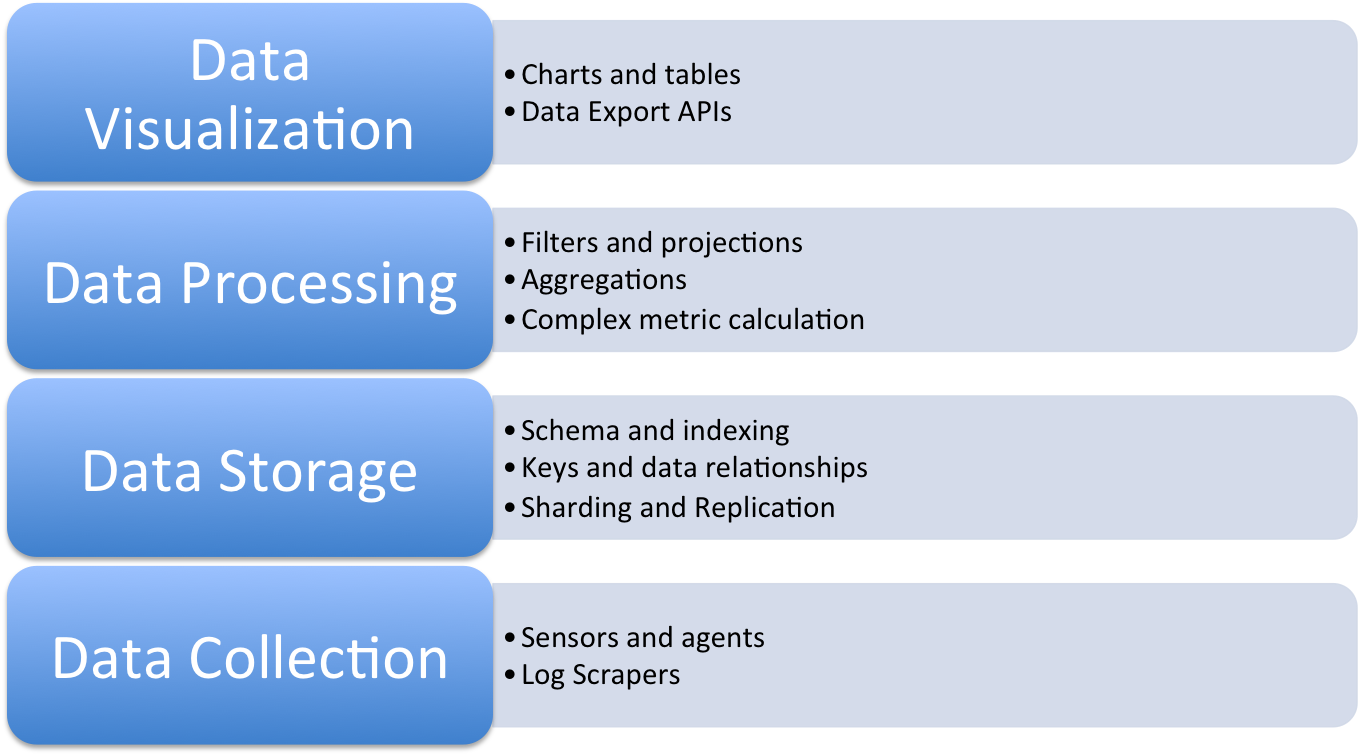
\includegraphics[scale=0.5]{apm_functions}
\caption{Key functions of the Roots APM.}
\label{fig:apm_functions}
\end{figure}

\begin{figure}
\centering
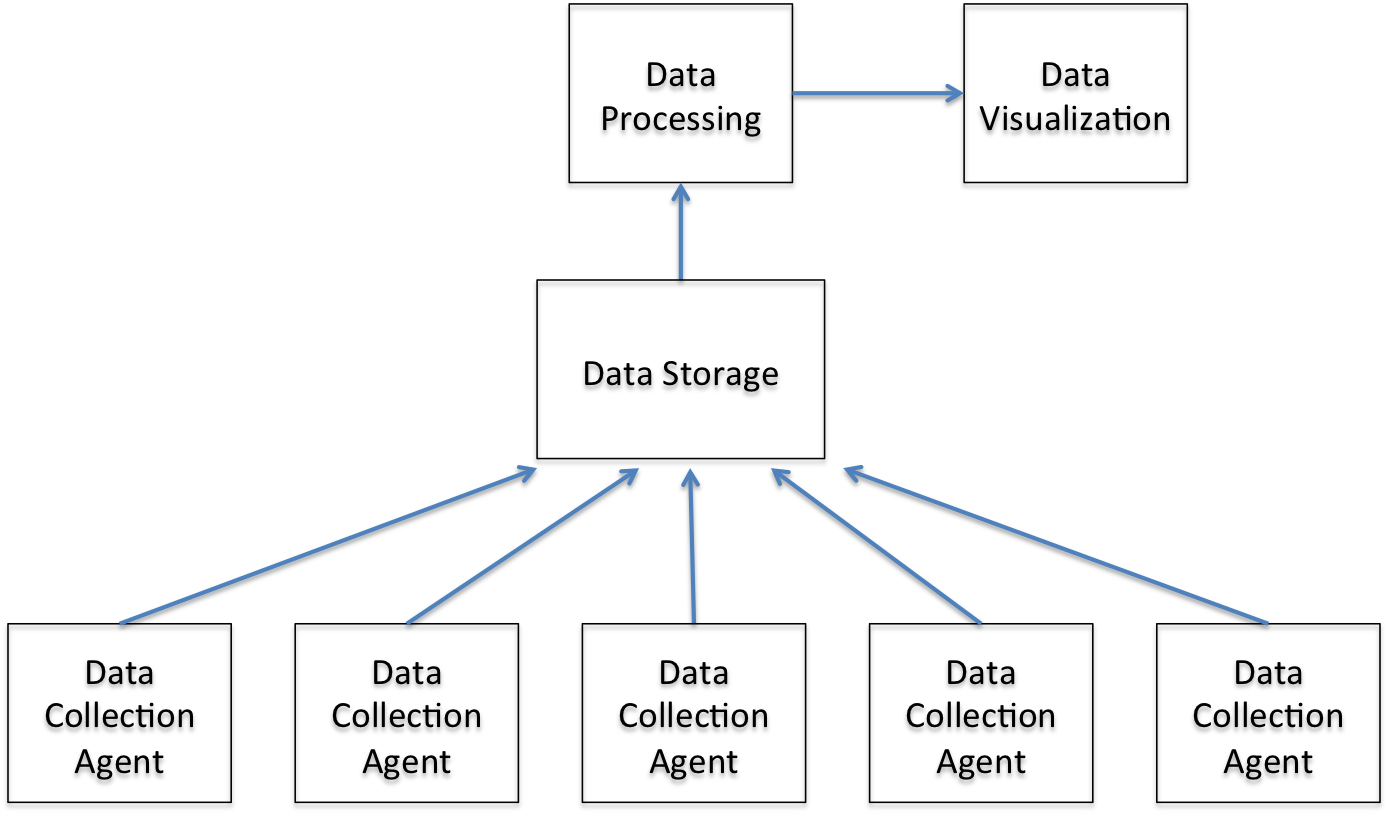
\includegraphics[scale=0.5]{apm_layout}
\caption{Deployment view of the Roots APM functions.}
\label{fig:apm_layout}
\end{figure}

Like most system monitoring solutions, the proposed cloud APM must serve four major functions: Data
collection, storage, processing (analytics) and visualization. Figure~\ref{fig:apm_functions} shows the
logical organization of these functions in the APM, and various tasks that fall under each of them.
Figure~\ref{fig:apm_layout} shows a physical deployment view of the said functions. Arrows indicate
the flow of information through the APM.

Data collection is performed by various sensors and agents that instrument the
core components of the PaaS cloud.
While sensors are very primitive in their capability to monitor
a given component, an agent may intelligently adapt to changing conditions, making decisions on
what information to capture and how often. 
Monitoring and instrumentation should be lightweight and as non-intrusive
as possible so their existence does not impose additional overhead 
on the applications. Specifically, we avoid instrumenting application code in Roots to prevent
introducing an additional overhead to the application execution. 

Data storage components should be capable of
dealing with potentially very high volumes of data. The data must be organized and indexed
to facilitate efficient retrieval, and replicated to maintain reliability and high availability. 
Additionally, Roots should also support timely removal of old data (i.e. garbage collection)
in an efficient and non-invasive manner.

Data processing components should also be capable of processing large volumes of data in near real-time,
while supporting a wide range of data analytics features such as filters, projections and aggregations. 
They will employ various statistical and perhaps even machine learning methods to understand the
data, detect anomalies and identify bottlenecks in the system. Roots should also provide high-level
abstractions so that new data analysis methods can be implemented when necessary.

Data visualization layer mainly consists of graphical interfaces (dashboards) for displaying various
metrics computed by the data processing components. Additionally it may also have APIs to export
the calculated results and trigger alerts. 

\subsubsection{APM Architecture and Integration with PaaS Clouds}
\begin{figure}
\centering
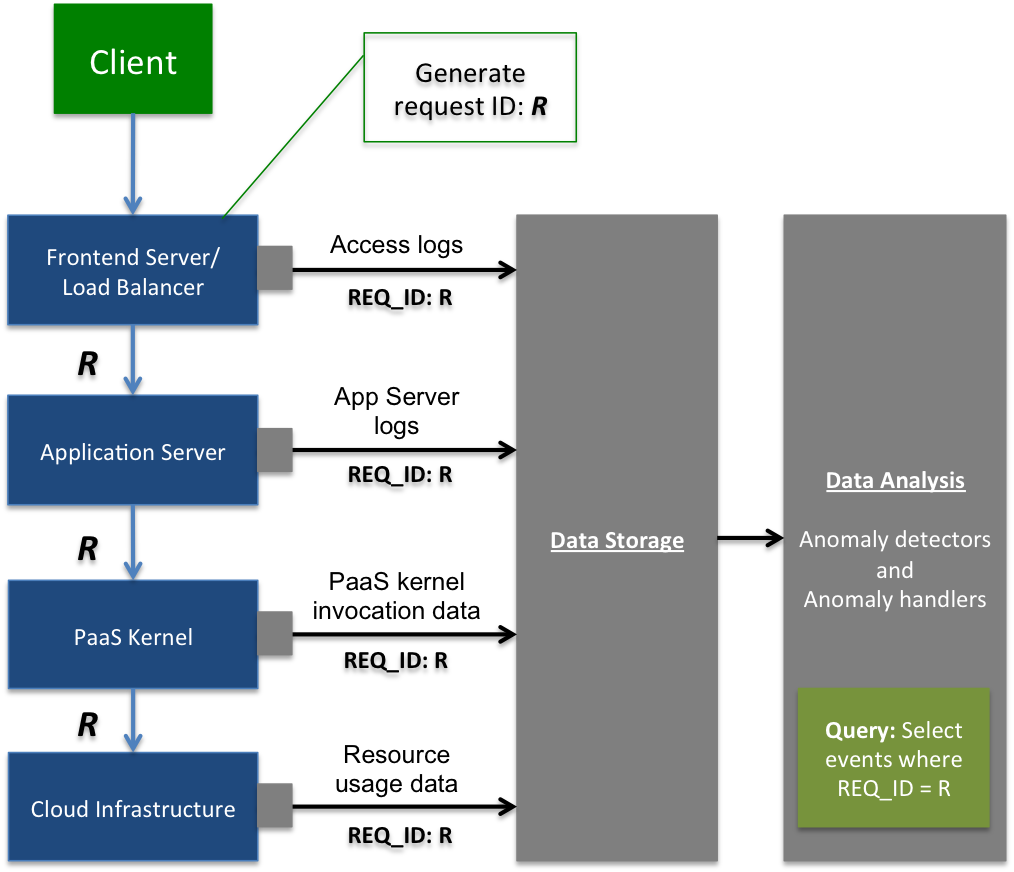
\includegraphics[scale=0.35]{apm_architecture}
\caption{APM architecture.}
\label{fig:apm_architecture}
\end{figure}

Figure~\ref{fig:apm_architecture} illustrates the overall architecture of the proposed APM, and how 
it fits into the PaaS cloud stack. APM components are shown in grey, with their interactions indicated
by the black lines. The small grey boxes attached to the PaaS components represent the sensors and
agents used to instrument the cloud platform for data collection purposes. Note that the APM collects
data from all layers in the PaaS stack (i.e. full stack monitoring).

From the front-end and load balancing layer we gather all information related to incoming application
requests. A big part of this is scraping the HTTP server access logs, which indicate request timestamps,
source and destination addressing information, response time (latency) and other HTTP message
parameters. This information is readily available for harvesting in most technologies used as front-end
servers (e.g. Apache HTTPD, Nginx). Additionally we may also collect information pertaining to active
connections, invalid access attempts and other errors.

From the application server layer we intend to collect basic application logs as well as any other logs and 
metrics that can be easily collected from the application runtime. This may include some process level
metrics indicating the resource usage of the individual application instances. Additionally Roots
employs a collection per-application benchmarking processes, that periodically probes applications
to measure their performance. These are lightweight, stateless processes managed by the Roots framework.
Data collected by these processes will also be sent to data storage component, and will be available
for analysis as per-application timeseries data.

At the PaaS kernel layer we employ instrumentation to record information regarding all kernel invocations
made by the applications. This instrumentation must be applied carefully as to not introduce a noticeable
overhead to the application execution. For each PaaS kernel invocation, we can capture the 
following parameters.
\begin{itemize}
\item Source application making the kernel invocation
\item Timestamp
\item Target kernel service and operation
\item Execution time of the invocation
\item Request size, hash and other parameters
\end{itemize}
Collecting this PaaS kernel invocation details enables tracing the execution of application 
requests, without the need for instrumenting application code, which we believe is a feature 
unique to PaaS clouds. 

Finally, at the lowest infrastructure level, we can collect information related to virtual machines, containers
and their resource usage. We can also gather metrics on network usage by individual components which
might be useful in a number of traffic engineering use cases. Where appropriate we can also scrape
hypervisor and container manager logs to get an idea of how resources are allocated and released over
time. However, we will not investigate data collected at this level in our immediate future work.
To begin with we wish to perform anomaly detection at the frontend and application server levels, and conduct
root cause analysis at the PaaS kernel level.

To summarize, the types of services and resources that Roots will be able
to monitor include the following. Moreover, our design of the Roots data collection 
layer is abstract and thus easily extended to permit monitoring of new services 
and PaaS components as they become available in the future.
\begin{itemize}
\item Cloud Infrastructure: 
  \begin{itemize}
  \item CPU, memory, disk, network
  \item Linux containers, virtual machines
  \end{itemize}
\item PaaS Kernel (including PaaS cloud SDK)
  \begin{itemize}
  \item Task queues, security components (user/developer tracking and authentication and authorization)
  \item Data caches, datastores (key value, NoSQL), databases (fixed schema, SQL).
  \end{itemize}
\item Application servers
  \begin{itemize}
  \item language-specific runtime systems
  \end{itemize}
\item Front-end components
  \begin{itemize}
  \item HTTP/S request serving 
  \item Load balancing and rate limiting components
  \end{itemize}
\end{itemize}

To avoid introducing delays to the application request processing flow, we implement
all Roots agents and sensors as asynchronous tasks. That is, none of them would
suspend application request processing to report data to the data storage components.
We make sure that all expensive I/O tasks related to data collection and storage is
executed out of the request processing flow.
In particular, all data is collected into log files or memory buffers that are local to the components being
monitored. This locally collected (or buffered) data will be periodically sent
to the data storage components of Roots using separate background tasks and batch communication
operations. Also special care is taken to isolate the activities in the cloud from potential
faults and failures in the Roots data collection or storage layers. 

\subsubsection{Cross-layer Data Correlation}
Previous subsection details how the APM collects useful monitoring data at each layer of the cloud
stack. To make most out of the gathered data, and use them to perform complex analyses, 
we must be able to correlate data records collected at different layers of the PaaS. For example consider
the execution of a single application request. This single event results in following data records at
different layers of the cloud, which will be collected and stored by the APM as separate entities.

\begin{itemize}
\item A front-end server access log entry
\item Zero or more application log entries
\item Zero or more PaaS kernel invocation records
\end{itemize}

We require a mechanism to tie these disparate records together, so the data processing layer can easily
aggregate the related information. For instance, we must be able to retrieve via an
aggregation query, all PaaS kernel invocations made by a specific application request.

To facilitate this requirement we propose that front-end server tags all incoming application requests 
with unique identifiers.
This request identifier can be attached to HTTP requests as a header which is visible to all components 
internal to the PaaS cloud. All data collecting agents can then be configured to record the request identifiers
whenever recording an event. At the data processing layer APM can aggregate the data by request identifiers
to efficiently group the related records.

\subsubsection{Data Analysis}
Roots data analysis layer uses two basic abstractions:
\begin{itemize}
\item Anomaly detector
\item Anomaly handler
\end{itemize}

Anomaly detectors are processes that periodically analyze the data collected for
each deployed application. Roots supports multiple detector implementations, where each implementation
uses a different statistical method to look for performance anomalies. Detectors are configured
at application level making is possible for different applications to use different anomaly 
detectors. Roots also supports multiple concurrent anomaly detectors on the same application, which can be used
to evaluate the efficiency of different detection strategies for any given application. Each
anomaly detector has an execution schedule (e.g. run every 60 seonds), and a sliding window 
(e.g. from 10 minutes ago to now)
associated with it. The boundaries and the length of the window determines the time range
of the data processed by the detector at any round of execution. Window is updated 
after each round of execution.

In addition to the various statistical anomaly detectors, Roots provides a special
``path anomaly detector'', that can be configured on any application. This detector
analyzes the sequences of PaaS SDK calls made by an application, and identifies the
different paths of execution that has resulted due to application request processing.
Each SDK call sequence corresponds to a path of execution through the application code.
This detector computes the frequency distribution of different paths (i.e. how often each path
gets executed), and checks how the distribution changes over time. By doing so the path anomaly
detector can identify the occurance of new paths (a type of novelty detection), most
frequently executed paths and
significant changes in the path frequency distribution. Such changes are usually
the results of changes in the nature of the application workload (e.g. from a readonly
workload to a readwrite workload in a data management application). 
This level of deep insight into application
performance and workload is possible in Roots only due to its systemwide data
collection and aggregation capabilities.

When an anomaly detector finds an anomaly in application performance, it sends an event
to a collection of anomaly handlers. The event encapsulates a unique anomaly identifier, 
timestamp, application identifier and the source detector's sliding window that correspond to the
anomaly. Anomaly handlers are configured globally (i.e. each handler
receives events from all detectors), but they can decide to not handle certain types
of anomaly events. Similar with detectors, Roots supports multiple anomaly handler
implementations -- one for logging anomalies, one for sending alert emails, one
for updating a dashboard etc. Additionally, Roots provides two special anomaly handler
implementations.
\begin{itemize}
\item Workload change analyzer
\item Root cause analyzer
\end{itemize}

The workload change analyzer analyzes the historical workload trends of the applications to
check if a particular anomaly is correlated with a recent change in the workload.
This is done by running a suite of changepoint detection algorithms on the workload
data captured by the Roots data collection layer. The root cause analyzer evaluates
the historical trend of PaaS SDK calls made by the application, and attempts to
determine the most likely components of the cloud (in the PaaS kernel) that may have 
attributed to a detected anomaly.

Both the anomaly detectors and anomaly handlers work with fix-sized sliding windows.
They are free to discard any old data as the sliding window moves along the time line.
As such the amount of state information these entities must keep in memory has
a strict upperbound. By doing so we make these processes lightweight. The old 
historical data can be kept persistently in the Roots data storage layer, until
they are deemed eligible for garbage collection.

The extensibility of Roots is primarily achieved through the abstractions of anomaly
detectors and handlers. Roots makes it simple to implement new detectors and handlers,
and plug them into the system. Both the detectors and the handlers are executed
as lightweight processes that do not interfere with the rest of the processes in
the cloud platform. Therefore failures in detectors and handlers have no impact
on the cloud platform or the deployed applications.

\subsubsection{Roots Process Management}
Most data collection activities in Roots can be treated as passive -- i.e. they
happen automatically as the applications receive and process requests in the cloud
platform. They do not require explicit scheduling or management. In contrast,
application benchmarking and data analysis are active processes that require
explicit scheduling and management.  This is achieved by grouping benchmarking
and data analysis processes into units called Roots pods. 

Each Roots pod is responsible for starting and maintainig a preconfigured set of
benchmarkers and data analysis processes (i.e. anomaly detectors and handlers). 
Each of these processes are light enough, so as to pack a large number of them
into a single pod. Pods are self-contained entities, and there is no inter-communication
between pods. Processes in a pod can efficiently communicate with each other 
(using shared memory), and call out to the Roots data storage to retrieve 
collected performance data for analysis. This enables starting and stopping 
Roots pods with minimal impact on the overall monitoring system. Furthermore, pods
can be replicated for high availability, and application load can be distributed
among multiple pods for scalability. For example, in a cloud platform with
1 million deployed applications, 100 pods can be used with each pod responsible
for running benchmarkers and analyzers for 10,000 applications.

To automate the process of managing pods, they can be tied into the core
process management framework of the PaaS cloud. That way whenever the cloud
platform initializes, a collection of pods can be started automatically.
Application deployment process of the PaaS cloud can be easily augmented
to register each new application with one of the available pods, so that the
benchmarkers and anomaly detectors can start running on the application.
Moreover, pods can be moved around or restarted as needed in response
to errors and autoscaling events that occur in the cloud platform.
